% !TEX TS-program = XeLaTeX

% STYLE

\documentclass[a4paper, 12pt]{article}
\usepackage[left=1in,
		    right=1in,
    		    top=1in,
		    bottom=1in,
		    bindingoffset=0cm]{geometry}
		    \usepackage{array}
\usepackage{float}
\usepackage{graphicx}
\graphicspath{ {./images/} }
\usepackage{subfig}
\usepackage{enumerate}
\usepackage[normalem]{ulem} % underlining
\usepackage{booktabs} % tables
\PassOptionsToPackage{table}{xcolor}% coloring tables
\providecommand{\keywords}[1]
{
  \small	
  \textbf{Keywords: }#1
}

% LANGUAGE + FONT
		    
\usepackage[english]{babel}
\usepackage[backend=biber,
                     style=unified]{biblatex}
\newcommand{\citeay}[2][]{\citeauthor{#2} (\citeyear[#1]{#2})}
\addbibresource{ref.bib}
\usepackage{fontspec}  
\setmainfont{Minion 3}
\usepackage{hyperref}
\hypersetup{
    colorlinks=true,
    linkcolor=black,
    citecolor=black,
    filecolor=black,
    urlcolor=blue,
}

% DRAWING

\usepackage{tikz}
\usepackage{tikz-qtree}
\usetikzlibrary{shapes.geometric}
\usetikzlibrary{trees,arrows}
\usetikzlibrary{positioning}
\usetikzlibrary{matrix}
\usetikzlibrary{tikzmark}
\usetikzlibrary{decorations.shapes}
\usetikzlibrary{shapes.misc}
 \usepackage{multirow}

% LINGUISTICS 

%\usepackage{gb4e}
\usepackage{expex}
\usepackage[glossaries]{leipzig}
\makeglossaries
\newleipzig {ipf} {ipf} {imperfective}
\newleipzig {npst} {npst} {non-past}
\newleipzig {lat} {lat} {lative case}
\newleipzig {cn} {cn} {connegative}
\newleipzig {freq} {freq} {frequentative}
\newleipzig {ill} {ill} {illative case}

\lingset{numoffset=0ex, textoffset=.6ex, belowglpreambleskip=0ex, aboveglftskip=0ex, belowexskip=2ex, aboveexskip=1ex}

\title{Moksha glide epenthesis}
\author{Sasha Shikunova}
\date{EGG 2023; last updated \today}

\begin{document}
\maketitle

	\section{Basic facts}
	
	Moksha < Mordvinic < Uralic, European part of Russia, Mordovia Republic and neighbouring regions; central dialect from Lesnoye Tsibaevo
	
	\begin{figure}[H]
		\centering
		\includegraphics[scale=.125]{mok-beginning}
		\hfill
		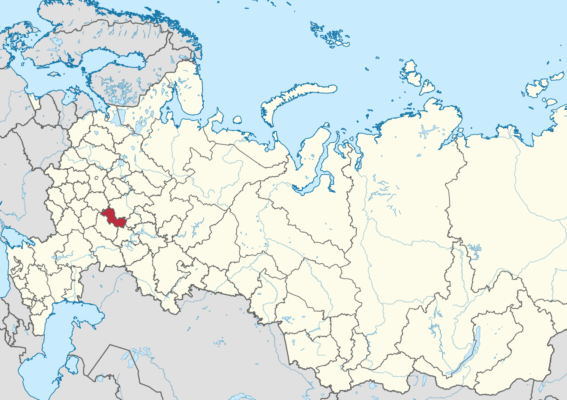
\includegraphics[scale=.373]{mok-map}
	\end{figure}
	
	\noindent Vowel and consonant inventories \parencite{kukhto2018}
	
\begin{minipage}{0.45\linewidth}

\begin{table}[H]
\begin{tabular}{cccccc}
\toprule
\multicolumn{2}{l}{i} &  & \multicolumn{2}{l}{(ɨ)} & u \\
e          & \multicolumn{3}{l}{(ɘ)}    & ə          & o \\
\multicolumn{2}{l}{ɛ} &  & \multicolumn{2}{l}{a}   &  \\
\bottomrule
\end{tabular}
\end{table}

\end{minipage}
\hfill
\begin{minipage}{0.45\linewidth}
\begin{table}[H]
\begin{tabular}{lllllll}
\toprule
m   &     & \begin{tabular}[c]{@{}l@{}}n\\ n'\end{tabular}      &                                                       &                                                  &    &     \\
p b &     & \begin{tabular}[c]{@{}l@{}}t d\\ t' d'\end{tabular} &                                                       &                                                  &    & k g \\
    & f v & \begin{tabular}[c]{@{}l@{}}s z\\ s' z'\end{tabular} &                                                       & \begin{tabular}[c]{@{}l@{}}š ž\\ šč\end{tabular} & j̊ & (x) \\
    &     & \begin{tabular}[c]{@{}l@{}}c\\ c'\end{tabular}      &                                                       & č                                                &    &     \\
    &     &                                                     &                                                       &                                                  & j  &     \\
    &     &                                                     & \begin{tabular}[c]{@{}l@{}}r̥ r\\ r̥' r'\end{tabular} &                                                  &    &     \\
    &     & l̥                                                  & l̥'                                                   &                                                  &    &     \\
    &     & l                                                   & l'                                                    &                                                  &    &    
\\
\bottomrule
\end{tabular}
\end{table}
\end{minipage}

	\begin{enumerate}[$\gg$]
		\item Contrastive palatalisation
		
			\pex 
				\a \emph{mar} -- \emph{mar'} \hfill `pile' -- `apple'
				\a \emph{kal} -- \emph{kal'} \hfill `fish' -- `willow'
			\xe
			
		\item Contrastive voicing in stops, fricatives and sonorants \parencite{kukhto2018}
		
			\pex
				\a \emph{katə} -- \emph{kadə} \hfill `cat' -- `leave.{\Cn}'
				\a \emph{t'asə} -- \emph{t'azə} \hfill `(be) here' -- `(come) here'
				\a \emph{mar̥'-n'ə} -- \emph{mar'-n'ə} \hfill `apple-{\Def}.{\Pl}' -- `apple-{\Fsg}.{\Poss}.{\Pl}'
			\xe
					
		\item /x/ only occurs in loanwords
		
			\pex 
				\a \emph{xul'igat-t'n'ə} \hfill `hooligan-{\Def}.{\Pl}'
				\a \emph{xalad'il'n'ək} \hfill `fridge'
			\xe
			
		\item {[ɨ]} is in complementary distribution with [i]: [i] after palatalised consonants, [ɨ] otherwise
		
			\ex \emph{ksti} [ɨ] -- \emph{kšt'i} [i] \hfill `berry' -- `dance.{\Cn}'
			\xe
		\item Schwa is fronted after palatalised consonants and becomes [ɘ]
		
			\ex \emph{mol'əms} [ɘ] \hfill `to go'
			\xe
		
	\end{enumerate}
	There are almost no restrictions on initial or final clusters in Moksha:
	
	\pex CC/CCC onsets
		\a \emph{kši} \hfill `bread'
		\a \emph{ksti} \hfill `berry'
		\a \emph{ftal} \hfill `back, behind'
	\xe
	
	\pex CC/CCC codas in non-derived words
		\a \emph{po\v{c}f} \hfill `flour'
		\a \emph{traks} \hfill `cow'
		\a \emph{ir̥'ks} \hfill `rib'
	\xe
	
	\pex~CCCC/CCCCC clusters on morpheme boundaries
		\a \emph{ir̥'ks-t} \hfill `rib-{\Pl}'
		\a \emph{kstikst} \hfill `berry garden.{\Pl}'
		\a \emph{bratksc'} \hfill `fraternise.{\Pst}.{\Tsg}'

	\xe
		
	The Moksha stress is conditioned by vowel quality \parencite{kukhto2018}. 
	
	\begin{enumerate}[$\gg$]
	\setlength\itemsep{0em}
		\item Syllables can be divided into \emph{heavy} (/a ɛ e o/ as nuclei) and \emph{light} (/u i ə/ as nuclei)
		\item Stress the leftmost heavy syllable
		\item In all-light words, stress falls on the leftmost syllable
	\end{enumerate}
		
		\vspace*{-1em}
\begin{minipage}[t]{.25\linewidth}
\ex\label{ex:tyadya}
	ˈt'ɛd'ɛ \\`mother'
\xe
\end{minipage}
\hfill
\begin{minipage}[t]{.25\linewidth}
\ex\label{ex:kuvakastress}
	kuˈvaka \\`long'
\xe
\end{minipage}	
\hfill
\begin{minipage}[t]{.4\linewidth}
\ex\label{ex:kijestress}
	ˈkijə \\`who'
\xe
\end{minipage}

	\noindent Even schwa can be stressable: in words where there are no heavy syllables
	
	\ex \emph{t{\'ə}rn-əs'-əm-s} \hfill `shiver-{\Freq}-{\Inf}-{\Ill}'
	\xe
	Stressed vowels are significantly longer than the unstressed ones; no reduction occurs in unstressed syllables.
		
		\section{Glide insertion}\label{sec:data}
		
	Sources of data: 
	
	\begin{enumerate}[$\gg$]
	\setlength\itemsep{0em}
		\item chapter on Moksha phonology by \citeay{kukhto2018}
		\item chapter on Moksha morphophonology by \citeay{kozlov2018}
		\item the \href{http://moksha.web-corpora.net}{Moksha corpus}
		\item online fieldwork
	\end{enumerate}
	Vowel hiatus is usually disallowed in Moksha. This is how it is escaped:
			
	\begin{enumerate}[$\gg$]
	\setlength\itemsep{0em}
		\item Glide insertion occurs after bases ending in /u/ or /i/ before vowel-initial suffixes \parencite{kozlov2018}
		\item No glide insertion after monosyllabic bases
		\item Different glide insertion rules before schwa- and /a/-initial suffixes (reduced vs full vowel)
	\end{enumerate}
				
			\subsection{Schwa-initial suffixes}
			
	 The glide epenthesis before schwa-initial suffixes inserts /v/ after /u/ (\ref{ex:u1}) and /j/ after /i/ (\ref{ex:u2}).\footnote{The part of the gloss in parentheses is not a part of the actual translation and serves to indicate that these forms are used as nominal predicates. The epenthetic /v/ and /j/ will be referred to as glides for the sake of simplicity, despite /v/ not being a glide.} After consonant-final bases the suffixal schwa is retained (\ref{ex:z1}, \ref{ex:z2}). There is no epenthesis after the unreduced vowels /a o e ɛ/ (\ref{ex:a1}, \ref{ex:a2}).
	
\begin{minipage}[t]{.3\linewidth}
\ex\label{ex:u1}
	jožu + əl' $\rightarrow$ jožuv-əl' \\`({\Tsg} was) smart-{\Ipf}'
\xe
\end{minipage}
\hfill
\begin{minipage}[t]{.315\linewidth}
\ex\label{ex:a1}
	ava + əl' $\rightarrow$ ava-l' \\`({\Tsg} was a) woman-{\Ipf}'
\xe
\end{minipage}	
\hfill
\begin{minipage}[t]{.33\linewidth}
\ex\label{ex:z1}
	ruz + əl' $\rightarrow$ ruzəl' \\`({\Tsg} was) Russian-{\Ipf}'
\xe
\end{minipage}

\begin{minipage}[t]{.3\linewidth}
\ex\label{ex:u2}
	t'ɛči + ən' $\rightarrow$ t'ɛčij-ən' \\`today-{\Gen}'
\xe
\end{minipage}	
\hfill
\begin{minipage}[t]{.315\linewidth}
\ex\label{ex:a2}
	ava + ən' $\rightarrow$ ava-n' \\`woman-{\Gen}'
\xe
\end{minipage}	
\hfill
\begin{minipage}[t]{.33\linewidth}
\ex\label{ex:z2}
	ruz + ən' $\rightarrow$ ruzən' \\`Russian-{\Gen}'
\xe
\end{minipage}
	
	\noindent As already mentioned, no epenthesis happens with monosyllabic bases, verbal or nominal (\ref{ex:mono1}--\ref{ex:mono2}).
	
\begin{minipage}[t]{.3\linewidth}
\ex\label{ex:mono1}
	ši + ən' $\rightarrow$ ši-n' \\`day-{\Gen}'
\xe
\end{minipage}
\hfill
\begin{minipage}[t]{.3\linewidth}
\ex\label{ex:}
	mu + əms $\rightarrow$ mu-ms \\`find-{\Inf}'
\xe
\end{minipage}	
\hfill
\begin{minipage}[t]{.3\linewidth}
\ex\label{ex:mono2}
	vi + əms $\rightarrow$ vi-ms \\`bring-{\Inf}'
\xe
\end{minipage}
	
	\noindent The behaviour of glides in between /u i/ and suffixal schwa is summarised in Table \ref{tab:glidesschwa} below. A\# corresponds to the unreduced vowels /a o e ɛ/.
	
\begin{table}[H]
\centering
\begin{tabular}{lllll}
\toprule
               & C\#                  & A\#                 & u\#  & i\#  \\
\midrule
monosyllabic      & \multirow{2}{*}{ən'} & \multirow{2}{*}{n'} & n'   & n'   \\
polysyllabic &                      &                     & vən' & jən'\\
\bottomrule
\end{tabular}
\caption{Suffix \emph{ən'} `{\Gen}' with different kinds of bases}
\label{tab:glidesschwa}
\end{table}
	
	\noindent The glide insertion is not synchronically productive -- it does not affect loanwords. The default strategy is to treat /u i/ exactly like other vowels: to drop the schwa altogether (\ref{ex:lw1}--\ref{ex:lw3}). The syllable count is of no importance with loanwords. 
	
\begin{minipage}[t]{.3\linewidth}
\ex\label{ex:lw1}
	žuri + ən' $\rightarrow$ žuri-n' \\`jury-{\Gen}'
\xe
\end{minipage}
\hfill
\begin{minipage}[t]{.3\linewidth}
\ex\label{ex:lw2}
	soči + ən' $\rightarrow$ soči-n' \\ `Sochi-{\Gen}' 
\xe
\end{minipage}	
\hfill
\begin{minipage}[t]{.3\linewidth}
\ex\label{ex:lw3}
	li + ən' $\rightarrow$ li-n' \\ `Li-{\Gen}'
\xe
\end{minipage}
				
			\subsection{/a/-initial suffixes}
			
	Suffixes that begin with /a/ cause glide epenthesis when attached to /u i/-final bases. Those are agreement markers \emph{-an} `{\Fsg}' and \emph{-at} `{\Ssg}' that can mark both verbal and nominal predicates \parencite{kholodilova-np, toldova-clauses}.
	
\begin{minipage}[t]{.45\linewidth}
\ex\label{ex:jozu}
	jožu + an $\rightarrow$ jožuvan \\`(I am) smart-{\Fsg}' 
\xe
\end{minipage}
\hfill
\begin{minipage}[t]{.45\linewidth}
\ex\label{ex:vidi}
	vidi + an $\rightarrow$ vidijan \\`(I am) a sower-{\Fsg}' 
\xe
\end{minipage}	

%	The interaction with bases ending in unreduced vowels and consonants is similar to the schwa-initial suffixes. The /a/ of the suffix is present after final consonants (\ref{}--\ref{})

	\noindent The peculiar property of the /a/-initial suffixes is that in monosyllabic bases ending in /u i/, no matter which vowel it is, /j/ is inserted at all times (\ref{ex:mu}--\ref{ex:li}).
	
\begin{minipage}[t]{.45\linewidth}
\ex\label{ex:mu}
	mu + an $\rightarrow$ mujan \\`(I) find-{\Fsg}' 
\xe
\end{minipage}
\hfill
\begin{minipage}[t]{.45\linewidth}
\ex\label{ex:li}
	li + an $\rightarrow$ lijan \\`(I) fly-{\Fsg}' 
\xe
\end{minipage}	

	\noindent Final /a ɛ/ coalesce with the suffix's vowel; as for the rest of the unreduced vowels -- /e o/ -- \citeay{kozlov2018} do not specify, only describing the phenomenon of `a-coalescence' with /a/ and /ɛ/ in base-final positions (\ref{ex:jaka}--\ref{ex:atya}). 
	
\begin{minipage}[t]{.45\linewidth}
\ex\label{ex:jaka}
	jaka + at $\rightarrow$ jakat \\`(you) go-{\Ssg}'
\xe
\end{minipage}
\hfill
\begin{minipage}[t]{.45\linewidth}
\ex\label{ex:atya}
	at'ɛ + an $\rightarrow$ at'an \\`(I am) an old man-{\Fsg}' 
\xe
\end{minipage}	

	\noindent Monosyllabic bases are different here again -- in single-syllable bases ending with /a/, no a-coalescence occurs and /j/ is inserted (\ref{ex:sa}--\ref{ex:shna}).
	
\begin{minipage}[t]{.45\linewidth}
\ex\label{ex:sa}
	sa + an $\rightarrow$ sajan \\`(I) come-{\Fsg}'
\xe
\end{minipage}
\hfill
\begin{minipage}[t]{.45\linewidth}
\ex\label{ex:shna}
	šna + an $\rightarrow$ šnajan \\`(I) praise-{\Fsg}'
\xe
\end{minipage}	

	The pattern is summarised in Table \ref{tab:glidesan}.
	
\begin{table}[H]
\centering
\begin{tabular}{lllll}
\toprule
              & C\#                 & A\# & u\# & i\#                  \\
\midrule
monosyllabic  & \multirow{2}{*}{an} & jan & jan & \multirow{2}{*}{jan} \\
polysyllabic &                     & n   & van &                     \\
\bottomrule
\end{tabular}
\caption{Suffix \emph{an} `{\Npst}.{\Fsg}' with different kinds of bases}
\label{tab:glidesan}
\end{table}

	\noindent Questions that we are going to answer:
	
	\begin{enumerate}[$\gg$]
		\item Is the syllable-counting rule reducible to something? In Strict CV phonology, flat and two-tiered, such rules are particularly difficult to implement.
		\item Where do the epenthetic glides come from?
			\begin{enumerate}[$\cdot$]
			\setlength\itemsep{0em}
				\item Floating segments?
				\item Spreading vowels?
			\end{enumerate}
		\item How do we model a distinction between reduced and full vowels wrt. glide insertion before them?
	\end{enumerate}
			
			\subsection{Suffixes starting with /u i/}
			
	There is one more phenomenon that is relevant to the glide insertion problem. Those are several suffixes in Moksha that start with a high vowel or consist of /u i/ alone, for instance, \emph{-i/j} `{\Npst}.{\Tsg}' and \emph{-u/v/i} `{\Lat}' \parencite{kozlov2018}.
	
\begin{minipage}[t]{.3\linewidth}
\ex\label{ex:jakaj}
	jaka-j `go-{\Tsg}' 
\xe
\end{minipage}
\hfill
\begin{minipage}[t]{.3\linewidth}
\ex\label{ex:shami}
	šam-i `empty-{\Tsg}' 
\xe
\end{minipage}	
	
\begin{minipage}[t]{.3\linewidth}
\ex\label{ex:mag}
	magazin-u \\`shop-{\Lat}'
\xe
\end{minipage}
\hfill
\begin{minipage}[t]{.3\linewidth}
\ex\label{ex:viri}
	vir'-i \\`forest-{\Lat}'
\xe
\end{minipage}	
\hfill
\begin{minipage}[t]{.3\linewidth}
\ex\label{ex:lavkav}
	lavka-v \\`shop-{\Lat}'
\xe
\end{minipage}

	\noindent The examples in (\ref{ex:jakaj}--\ref{ex:lavkav}) show that it is not out of the ordinary for /u i/ in Moksha to alternate with the corresponding glides. The glide insertion is not the only process where these alternations are observable, hence an analysis that can handle the /u i/-suffixes pattern on par with the glide insertion is preferable.
		
		\section{Glide epenthesis is conditioned by stress}\label{sec:proposal}

	The gist of my proposal:
	\begin{enumerate}[$\gg$]
%	\setlength\itemsep{0em}
		\item Heavy vowels /a o ɛ e/ and the stressed light vowels /u i ə/ are long; in Strict CV terms, they are associated to two CV slots
		\item The stress falls on the leftmost long vowel, and where there are no long vowels, an empty CV is inserted to the right of the leftmost vowel so that it is lengthened
		\item Therefore base-final /a o ɛ e/ and final /u i ə/ in monosyllabic bases form a natural class: they end in a long vowel
	\end{enumerate}
	
		\begin{minipage}{0.5\linewidth}
			\ex\label{fig:kuvaka} {[kuˈvaka]} \\
				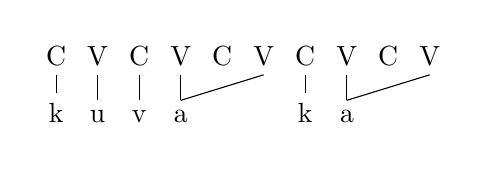
\begin{tikzpicture}
\matrix [matrix of nodes, row sep=0.1em,
column sep={1.5em,between origins}]
{
|(c1)|{C} & |(v1)|{V} & |(c2)|{C} & |(v2)|{V} & |(c3)|{C} & |(v3)|{V} & |(c4)|{C} & |(v4)|{V} & |(c5)|{C} & |(v5)|{V}      \\[0.6em]
|(C1)|{k} & |(V1)|{u} & |(C2)|{v} & |(V2)|{a} & |(C3)|{} & |(V3)|{} & |(C4)|{k} & |(V4)|{a} & |(C5)|{} & |(V5)|{} \\
};
\draw (c1.south) -- (C1.north);
\draw (v1.south) -- (V1.north);
\draw (c4.south) -- (C4.north);
\draw (v4.south) -- (V4.north);
\draw (v5.south) -- (V4.north);
\draw (c2.south) -- (C2.north);
\draw (v2.south) -- (V2.north);
\draw (v3.south) -- (V2.north);
				\end{tikzpicture}
			\xe
		\end{minipage}
	\hfill	
		\begin{minipage}{0.4\linewidth}
			\ex\label{fig:kije} {[ˈkijə]} \\
				\begin{tikzpicture}
\matrix [matrix of nodes, row sep=0.1em,
column sep={1.5em,between origins}]
{
|(c1)|{C} & |(v1)|{V} & |(c2)|{C} & |(v2)|{V} & |(c3)|{C} & |(v3)|{V}      \\[0.6em]
|(C1)|{k} & |(V1)|{i} & |(C2)|{} & |(V2)|{} & |(C3)|{j} & |(V3)|{ə} \\
};
\draw (c1.south) -- (C1.north);
\draw (v1.south) -- (V1.north);
\draw (c3.south) -- (C3.north);
\draw (v2.south) -- (V1.north);
\draw (v3.south) -- (V3.north);
				\end{tikzpicture}
			\xe
		\end{minipage}
		
	\begin{enumerate}[$\gg$]
%	\setlength\itemsep{0em}
		\item The glide insertion is the result of /u i/ spreading onto the initial C of the suffix
		\item Long vowels do not spread
		\item The restriction on triple association, or extra-long segments, is widely attested and may be universal \parencite{chekayri-scheer2004, enguehard2018}
	\end{enumerate}
	
\begin{minipage}[t]{.4\linewidth}
			\ex\label{fig:shin} ši + ən' $\rightarrow$ {[ši-n']} \\
				\begin{tikzpicture}
\matrix [matrix of nodes, row sep=0.1em,
column sep={1.5em,between origins}]
{
|(c1)|{C} & |(v1)|{V} & |(c2)|{C} & |(v2)|{V} & |(c4)|{--} & |(c3)|{C} & |(v3)|{V} & |(c5)|{C} & |(v5)|{V}      \\[0.6em]
|(C1)|{š} & |(V1)|{i} & |(C2)|{} & |(V2)|{} & |(C4)|{} & |(C3)|{} & |(V3)|{ə} & |(C5)|{n'} & |(V5)|{} \\
};
\draw (c1.south) -- (C1.north);
\draw (v1.south) -- (V1.north);
\draw (v2.south) -- (V1.north);
\draw (c5.south) -- (C5.north);
\draw (v3.south) -- (V3.north);
\draw[->] (V1.east) -- node[strike out,draw,-]{} (c3.south);
				\end{tikzpicture}
			\xe
\end{minipage}
\hfill
\begin{minipage}[t]{.5\linewidth}
			\ex\label{fig:tyachi} t'ɛči + ən' $\rightarrow$ {[t'ɛčij-ən']} \\
				\begin{tikzpicture}
\matrix [matrix of nodes, row sep=0.1em,
column sep={1.5em,between origins}]
{
|(c1)|{C} & |(v1)|{V} & |(c2)|{C} & |(v2)|{V} & |(c3)|{C} & |(v3)|{V} & |(c)|{--} & |(c4)|{C} & |(v4)|{V} & |(c5)|{C} & |(v5)|{V}      \\[0.6em]
|(C1)|{t'} & |(V1)|{ɛ} & |(C2)|{} & |(V2)|{} & |(C3)|{č} & |(V3)|{i} & |(C)|{} & |(C4)|{} & |(V4)|{ə} & |(C5)|{n'} & |(V5)|{} \\
};
\draw (c1.south) -- (C1.north);
\draw (v1.south) -- (V1.north);
\draw (v2.south) -- (V1.north);
\draw (c3.south) -- (C3.north);
\draw (v3.south) -- (V3.north);
\draw (c5.south) -- (C5.north);
\draw (v4.south) -- (V4.north);
\draw[->] (V3.north) -- (c4.south);
				\end{tikzpicture}
			\xe
\end{minipage}	

	\noindent The schwa disappears after long vowels and stays after consonants, be it base-final consonants or glides that appear after spreading. I suggest that schwa is deleted rather via coalescence with the long vowel than as a result of some vowel-zero alternation, because, should there be a vowel-zero alternation, we would expect the schwa to disappear after C\# as well.
	
	I now turn to two other previously described phenomena: (a) the vowel-glide alternation in /u i/-suffixes; (b) /j/-insertion in between monosyllabic bases with a heavy syllable and an /a/-initial suffix.
			
			\subsection{/u i/-suffixes are consonants}
			
	I argue that a similar analysis based on of /u i/ associating to two slots (C and V) can be pursued for the /u i/-initial suffixes, albeit with a change in representations: the /u i/ of these suffixes are better conceived of as underlying consonants.
	
\begin{minipage}[t]{.45\linewidth}
			\ex\label{fig:shami} {[šam-i]} \\
				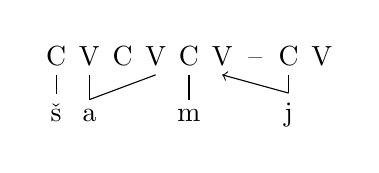
\begin{tikzpicture}
\matrix [matrix of nodes, row sep=0.1em,
column sep={1.2em,between origins}]
{
|(c2)|{C} & |(v2)|{V} & |(c21)|{C} & |(v21)|{V} & |(c3)|{C} & |(v3)|{V} & |(c)|{--} & |(c4)|{C} & |(v4)|{V}     \\[0.6em]
|(C2)|{š} & |(V2)|{a} & |(C21)|{} & |(V21)|{} & |(C3)|{m} & |(V3)|{} & |(C)|{} & |(C4)|{j} & |(V4)|{} \\
};
\draw (c2.south) -- (C2.north);
\draw (v2.south) -- (V2.north);
\draw (v21.south) -- (V2.north);
\draw (c3.south) -- (C3.north);
\draw (c4.south) -- (C4.north);
\draw[->] (C4.north) -- (v3.south);
				\end{tikzpicture}
			\xe
\end{minipage}
\hfill
\begin{minipage}[t]{.45\linewidth}
			\ex\label{fig:jakaj} {[jaka-j]} \\
				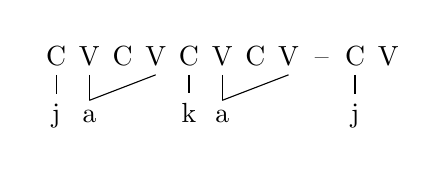
\begin{tikzpicture}
\matrix [matrix of nodes, row sep=0.1em,
column sep={1.2em,between origins}]
{
|(c2)|{C} & |(v2)|{V} & |(c21)|{C} & |(v21)|{V} & |(c3)|{C} & |(v3)|{V} & |(c31)|{C} & |(v31)|{V} & |(c)|{--} & |(c4)|{C} & |(v4)|{V}     \\[0.6em]
|(C2)|{j} & |(V2)|{a} & |(C21)|{} & |(V21)|{} & |(C3)|{k} & |(V3)|{a} & |(C31)|{} & |(V31)|{} & |(C)|{} & |(C4)|{j} & |(V4)|{} \\
};
\draw (c2.south) -- (C2.north);
\draw (v2.south) -- (V2.north);
\draw (v21.south) -- (V2.north);
\draw (c3.south) -- (C3.north);
\draw (v3.south) -- (V3.north);
\draw (v31.south) -- (V3.north);
\draw (c4.south) -- (C4.north);
%\draw[->] (V3.north) -- (c4.south);
				\end{tikzpicture}
			\xe
\end{minipage}	
	
	\noindent With the vowel associated, the analysis gets in conflict with the behaviour of another alternating suffix \emph{u/əv} `{\Pass}', which occurs as \emph{-(ə)v} before and/or after vowels (\ref{ex:savan}--\ref{ex:ucheva}) and is in free variation between \emph{-u} and \emph{-əv} in between consonants (\ref{ex:alternating}). 
	
\begin{minipage}[t]{.3\linewidth}
\ex\label{ex:savan}
	sa-v-an \\`come-{\Pass}-{\Npst}.{\Fsg}'
\xe
\end{minipage}
\hfill
\begin{minipage}[t]{.3\linewidth}
\ex\label{ex:ucheva}
	uč-əv-ə \\`wait-{\Pass}-{\Cn}' 
\xe
\end{minipage}	
\hfill
\begin{minipage}[t]{.3\linewidth}
\ex\label{ex:alternating}
	šav-əv-s' $\sim$ šav-u-s' \\ `kill-{\Pass}-{\Pst}.{\Tsg}'
\xe
\end{minipage}	
	
	\noindent Should its underlying representation be \emph{-u}, its shapeshifting in the presence of vowels would require reassociating it to a C-slot so as to free up a V-slot for the next vowel to associate to. With the suffix as a consonant, on the other hand, the analysis is more elegant and capable of capturing the variation between \emph{-u} and \emph{-əv} in between consonants: either there is association to the free base-final V (\ref{fig:shavus}) or not (\ref{fig:shavavs}).\footnote{I leave the exact Government-based mechanism of schwa insertion to future research, however, it can be noted that final empty nuclei are able to govern, since there are numerous examples of word-final clusters (for instance, \emph{satfks} `success', \emph{lifkst} `smallpox').}
%	Also, the schwa in \ref{fig:shavavs} is not inserted as a means of dissimilation: cf. \emph{}.
	
\begin{minipage}[t]{.45\linewidth}
			\ex\label{fig:shavus} {[šav-u-s']} \\
				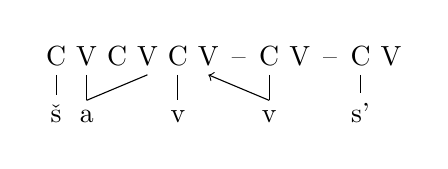
\begin{tikzpicture}
\matrix [matrix of nodes, row sep=0.1em,
column sep={1.1em,between origins}]
{
|(c2)|{C} & |(v2)|{V} & |(c21)|{C} & |(v21)|{V} & |(c3)|{C} & |(v3)|{V} & |(c)|{--} & |(c4)|{C} & |(v4)|{V} & |(c)|{--} & |(c5)|{C} & |(v5)|{V}     \\[0.6em]
|(C2)|{š} & |(V2)|{a} & |(C21)|{} & |(V21)|{} & |(C3)|{v} & |(V3)|{} & |(C)|{} & |(C4)|{v} & |(V4)|{} & |(C)|{} & |(C5)|{s'} & |(V5)|{} \\
};
\draw (c2.south) -- (C2.north);
\draw (v2.south) -- (V2.north);
\draw (v21.south) -- (V2.north);
\draw (c3.south) -- (C3.north);
\draw (c4.south) -- (C4.north);
\draw (c5.south) -- (C5.north);
\draw[->] (C4.north) -- (v3.south);
				\end{tikzpicture}
			\xe
\end{minipage}
\hfill
\begin{minipage}[t]{.45\linewidth}
			\ex\label{fig:shavavs} {[šav-əv-s']} \\
				\begin{tikzpicture}
\matrix [matrix of nodes, row sep=0.1em,
column sep={1.1em,between origins}]
{
|(c2)|{C} & |(v2)|{V} & |(c21)|{C} & |(v21)|{V} & |(c3)|{C} & |(v3)|{V} & |(c)|{--} & |(c4)|{C} & |(v4)|{V} & |(c)|{--} & |(c5)|{C} & |(v5)|{V}     \\[0.6em]
|(C2)|{š} & |(V2)|{a} & |(C21)|{} & |(V21)|{} & |(C3)|{v} & |(V3)|{ə} & |(C)|{} & |(C4)|{v} & |(V4)|{} & |(C)|{} & |(C5)|{s'} & |(V5)|{} \\
};
\draw (c2.south) -- (C2.north);
\draw (v2.south) -- (V2.north);
\draw (v21.south) -- (V2.north);
\draw (c3.south) -- (C3.north);
\draw (c4.south) -- (C4.north);
\draw (c5.south) -- (C5.north);
\draw[->] (C4.north) -- node[strike out,draw,-]{} (v3.315);
\draw[->] (V3.north) -- (v3.south);
\draw [->] (v4.north) -- ++(north:2.5ex) -| (v3.north) node[midway,above]  {G} node[pos=0.3,sloped,rotate=45]{$|$}node[pos=0.3,sloped,rotate=45]{$|$};
				\end{tikzpicture}
			\xe
\end{minipage}	
						
			\subsection{Are glides floating segments?}
			
	Arguments in favour of representing glides as floating segments:
	\begin{enumerate}[$\gg$]
	\setlength\itemsep{0em}
		\item Glide insertion is not synchronically productive: it never happens in loanwords, no matter their syllable count or stress pattern
		\item The glides that appear in glide insertion are historically recoverable \parencite[pp. 11--12]{bubrikh1953}
		\item There is a native Moksha exception to the rule -- \emph{ksti} `berry', which does cause glide insertion in spite of being monosyllabic \parencite[p. 42]{kozlov2018}
	\end{enumerate}
				
\begin{minipage}[t]{.3\linewidth}
\ex\label{ex:lw1s}
	žuˈri + ən' $\rightarrow$ žuri-n' \\`jury-{\Gen}' 
\xe
\end{minipage}
\hfill
\begin{minipage}[t]{.3\linewidth}
\ex\label{ex:lw2s}
	ˈsoči + ən' $\rightarrow$ soči-n' \\ `Sochi-{\Gen}'
\xe
\end{minipage}	
\hfill
\begin{minipage}[t]{.3\linewidth}
\ex\label{ex:lw3s}
	li + ən' $\rightarrow$ li-n' \\ `Li-{\Gen}'
\xe
\end{minipage}
		
	\noindent Finally, the rule that determines stress placement is not productive either on relatively fresh loanwords -- see the examples of Russian loanwords in (\ref{ex:krushka}--\ref{ex:kniga}), which do not obey the law of stressing the leftmost heavy syllable.
	
\begin{minipage}[t]{.45\linewidth}
\ex\label{ex:krushka}
	ˈkruška `cup'
\xe
\end{minipage}
\hfill
\begin{minipage}[t]{.45\linewidth}
\ex\label{ex:kniga}
	ˈkniga `book'
\xe
\end{minipage}	

	\noindent The analysis that links stress and glide epenthesis is therefore not incoherent: both rules are not extendable to loanwords, so the link between them is plausible. At the moment in the history of Moksha when both of them were productive, the connection that I have established might well have held.
	
			\subsection{Monosyllabic bases -- always with glides?}
		
\begin{minipage}[t]{.45\linewidth}
\ex\label{ex:sa1}
	sa + an $\rightarrow$ sajan \\`come-{\Fsg}' \\ \parencite[p. 57]{kozlov2018}
\xe
\end{minipage}
\hfill
\begin{minipage}[t]{.45\linewidth}
\ex\label{ex:shna1}
	šna + an $\rightarrow$ šnajan \\`praise-{\Fsg}' 
\xe
\end{minipage}	

\begin{minipage}[t]{.45\linewidth}
\ex\label{ex:mu1}
	mu + an $\rightarrow$ mujan \\`find-{\Fsg}' 
\xe
\end{minipage}
\hfill
\begin{minipage}[t]{.45\linewidth}
\ex\label{ex:li1}
	li + an $\rightarrow$ lijan \\`fly-{\Fsg}' 
\xe
\end{minipage}	
	
	\begin{enumerate}[$\gg$]
		\item The /j/ inserted in between heavy vowels has nothing to do with stress
		\item Heavy vowels like /a/, on the other hand, \emph{can} be base-final and stressed if there are no other heavy vowels on their left
	\end{enumerate}
	
\ex\label{ex:juma}
	juma + an $\rightarrow$ juman \\`(I am) lost-{\Fsg}' 
\xe

	\noindent Therefore, the /j/-insertion in monosyllabic /a/-final bases can be analysed as an effect of a floating segment without detriment to any generalisations already posited. 
	
	\begin{enumerate}[$\gg$]
		\item Suppose there is a floating glide after every monosyllabic base
		\item The glide only surfaces before unreduced vowels
		
\ex\label{ex:shtajan}
	šta + an $\rightarrow$ štajan \\`wash-{\Fsg}' 
\xe
		
		\item It is deleted before consonants, before schwa and word-finally
		
\begin{minipage}[t]{.3\linewidth}
\ex\label{ex:shtas}
	šta + s' $\rightarrow$ štas' \\`wash-{\Pst}.{\Tsg}' 
\xe
\end{minipage}
\hfill
\begin{minipage}[t]{.34\linewidth}
\ex\label{ex:izsa}
	iz' sa \\`{\Neg}.{\Pst}.{\Tsg} come.{\Cn}'
\xe
\end{minipage}	
\hfill
\begin{minipage}[t]{.3\linewidth}
\ex\label{ex:sal}
	sa + əl' $\rightarrow$ sal' \\`come-{\Ipf}'
\xe
\end{minipage}

	\end{enumerate}	
	
	\noindent We have to restrict the floating glide's ability to associate: it can only associate to a licensed position. Schwa cannot licence the preceding C-slot (\ref{fig:sal}), whereas /a/ can (\ref{fig:sajanlic}).
	
\begin{minipage}[t]{.45\linewidth}
			\ex\label{fig:sal} sa + əl' {[sa-l']} \\
				\begin{tikzpicture}
\matrix [matrix of nodes, row sep=0.1em,
column sep={1.5em,between origins}]
{
|(c2)|{C} & |(v2)|{V}  & |(c)|{--} & |(c4)|{C} & |(v4)|{V} & |(c5)|{C} & |(v5)|{V}     \\[0.6em]
|(C2)|{s} & |(V2)|{a} & |(C)|{j} & |(C4)|{} & |(V4)|{ə} & |(C5)|{l'} & |(V5)|{} \\
};
\draw (c2.south) -- (C2.north);
\draw (v2.south) -- (V2.north);
\draw (v4.south) -- (V4.north);
\draw (c5.south) -- (C5.north);
\draw [->] (v4.north) -- ++(north:2.5ex) -| (c4.north) node[midway,above]  {L} node[pos=0.3,sloped,rotate=135]{$|$}node[pos=0.3,sloped,rotate=135]{$|$};
				\end{tikzpicture}
			\xe
\end{minipage}
\hfill
\begin{minipage}[t]{.45\linewidth}
			\ex\label{fig:sajanlic} sa + an {[sa-jan]} \\
				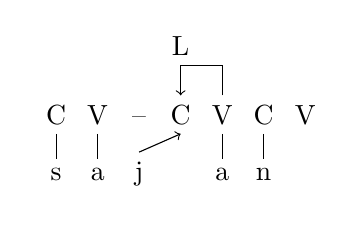
\begin{tikzpicture}
\matrix [matrix of nodes, row sep=0.1em,
column sep={1.5em,between origins}]
{
|(c2)|{C} & |(v2)|{V}  & |(c)|{--} & |(c4)|{C} & |(v4)|{V} & |(c5)|{C} & |(v5)|{V}     \\[0.6em]
|(C2)|{s} & |(V2)|{a} & |(C)|{j} & |(C4)|{} & |(V4)|{a} & |(C5)|{n} & |(V5)|{} \\
};
\draw (c2.south) -- (C2.north);
\draw (v2.south) -- (V2.north);
\draw (v4.south) -- (V4.north);
\draw (c5.south) -- (C5.north);
\draw[->] (C.north) -- (c4.south);
\draw [->] (v4.north) -- ++(north:2.5ex) -| (c4.north) node[midway,above] {L};				
				\end{tikzpicture}
			\xe
\end{minipage}	
	
	\begin{enumerate}[$\gg$]
%	\setlength\itemsep{0em}
		\item In /u i/-final monosyllabic bases, /j/ is inserted before /a/ but nothing is inserted before schwa
		\item /u i/-final monosyllabic bases act exactly like the /a/-final ones
		\item They may have the same floating glide that associates before full vowels (in licensed positions)
		\item The glide, however, cannot associate before schwa: recall that it is lost in \emph{sa<j> + əl'} $\rightarrow$ \emph{sal'}
		\item We still need an explanation of why /u i/ can't spread in monosyllabics
	\end{enumerate}
					
			\subsection*{IPA correspondence table \vspace*{-1em}}
			
\begin{minipage}[t]{.3\linewidth}
\begin{table}[H]
\begin{tabular}{cc}
\toprule
IPA        & Transcription \\
\bottomrule
m          & m                       \\
n̪         & n                       \\
n̪\textsuperscript{j}        & n'                      \\
p          & p                       \\
b          & b                       \\
t̪         & t                       \\
t̪\textsuperscript{j}        & t'                      \\
d̪         & d                       \\
d̪\textsuperscript{j}        & d'                      \\
k          & k                       \\
g          & g                       \\
x          & x                       \\
f (ɸ)      & f                       \\
     &                  \\
     \addlinespace[0.065cm]
\bottomrule
\end{tabular}
\end{table}
\end{minipage}
\hfill
\begin{minipage}[t]{.3\linewidth}
\begin{table}[H]
\begin{tabular}{cc}
\toprule
IPA        & Transcription \\
\bottomrule
v (β)      & v                       \\
s̪         & s                       \\
s̪\textsuperscript{j}        & s'                      \\
z̪         & z                       \\
z̪\textsuperscript{j}         & z'                      \\
ʃ          & š                       \\
ʃ\textsuperscript{j}ː (ʃt͡ʃ) & šč                      \\
ʒ          & ž                       \\
t͡s̪       & c                       \\
t͡s̪\textsuperscript{j}      & c'                      \\
t͡ʃ        & č                       \\
ç         & j̊                      \\
j          & j                       \\
ɾ̥         & r̥                      \\
\bottomrule
\end{tabular}
\end{table}
\end{minipage}	
\hfill
\begin{minipage}[t]{.3\linewidth}
\begin{table}[H]
\begin{tabular}{cc}
\toprule
IPA        & Transcription \\
\bottomrule
ɾ̥\textsuperscript{j}        & r̥'                     \\
ɾ          & r                       \\
ɾ\textsuperscript{j}         & r'                      \\
ɬ̪         & l̥                      \\
ɬ̪\textsuperscript{j}        & l̥'                     \\
l̪         & l                       \\
l\textsuperscript{j}        & l'                      \\
i          & i                       \\
u          & u                       \\
e          & e                       \\
ə          & ə                       \\
o          & o                       \\
ɛ          & ɛ                       \\
a          & a                      \\
\addlinespace[0.065cm]
\bottomrule
\end{tabular}
\end{table}
\end{minipage}	

\newpage
			\subsection*{List of glossing abbreviations \vspace*{-1.5em}}
			
\begin{multicols}{2}
\printglossary[title={}, style=mcolindex, nonumberlist]
\end{multicols}

\printbibliography
\end{document}